% !TEX root=../../Thesis.tex
\chapter{Modeling Intersection Driving Scenarios}
\label{ch:modeling_intersection}
\tommy{modeling is the key to...}
\begin{center}
  \textit{\textbf{RQ 1: How can RL be used to create a decision-making agent for autonomous driving through an unsignalized intersection?}}
  \end{center}
  \vspace{12pt}
  
Driving through an intersection is a sequential decision making problem and can be mathematically formulated using a \gls{mdp}, introduced in Section~\ref{sec:background_mdp}, but because the intention of other drivers is not observable with any existing sensors today, \gls{pomdp} is better suited to formulate the problem. 
\Citet{Shalev2016} raises two concerns when using Machine learning, specially Reinforcement learning, for autonomous driving applications: ensuring functional safety of the Driving Policy and that the Markov Decision Process model is problematic, because of unpredictable behavior of other drivers.
In the real world, intentions of other drivers are not always deterministic or predefined. Depending on their intention, different actions can be chosen to give the most comfortable and safe passage through an intersection.
They also noted that in the context of autonomous driving, the dynamics of vehicles is Markovian but the behavior of other road users may not necessarily be Markovian.

This Chapter defines the \gls{pomdp} for the intersection studied in this thesis. 

\section{Intersection scenarios}

% \begin{figure}
% \centering
% \begin{tikzpicture}

% 	% Crossing
% 	\def\crosstopy{8}
% 	\def\crossboty{-2.5}
% 	\def\crossleftx{-7}
	
% 	\draw[thick] (\crossleftx, 1) -- (-1, 1) -- (-1, \crosstopy);
% 	\draw[thick] (\crossleftx, -1) -- (-1, -1) -- (-1, \crossboty);
% 	\draw[thick] (1, \crosstopy) -- (1, 1) -- (3, 1);
% 	\draw[thick] (1, \crossboty) -- (1, -1) -- (3, -1);
	
% 	cars
% 	\node[inner sep=0pt] (ego_car) at (-6,0)
% 	{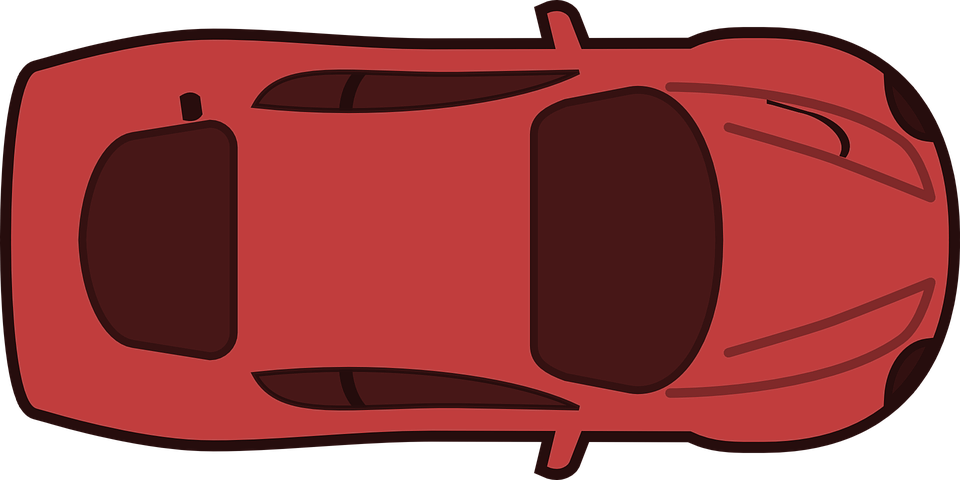
\includegraphics[width=.18\textwidth, angle=0]{figures/ego_car_top_down.png}};
% 	\draw[->] ([yshift=0.2cm]ego_car.east) -- node[above] {$v^{ego}$} ($ (ego_car) + (2,0.2)$ );
% 	\draw[|-|] ([yshift=-0.2cm]ego_car.east) -- node[below] {$p^{ego}_{0}=v^{ego}*\tau_{int}$} (-1,-0.2);

% 	\node[inner sep=0pt] (target_car_3) at (0,7)
% 	{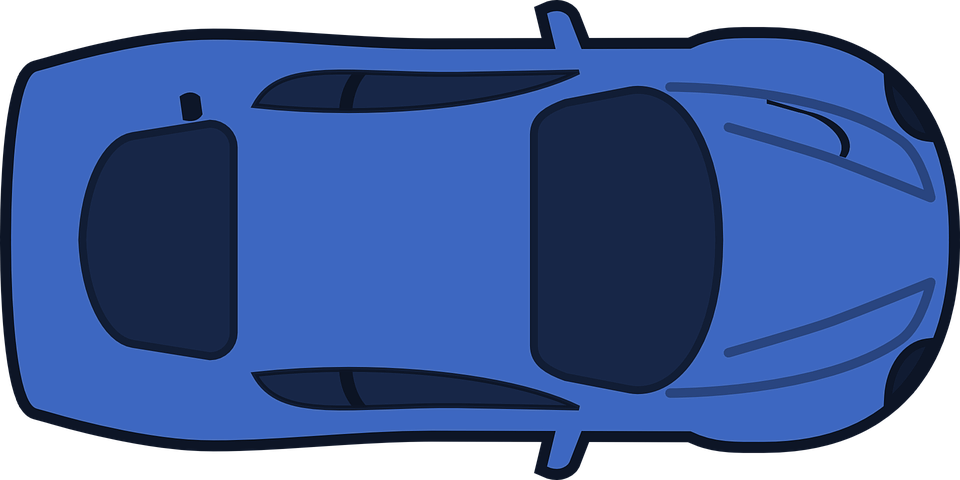
\includegraphics[width=.18\textwidth, angle=-90]{figures/target_car_top_down.png}};
% 	\node (tc_text3a) [right=of target_car_3, align=center] {Car 3};
% 	\node (tc_text3b) [left=of target_car_3, align=center] {Conflict Car};
% 	\draw[->] ([xshift=0.3cm]target_car_3.south) -- node[right] {$v^{3}_0$} ($ (target_car_3) + (.3,-2)$ );
% 	\draw[|-|] ([xshift=-0.8cm]target_car_3.south) -- (-.8,1);
% 	\node (tc_tti) [below left= 0.9cm and -0.7cm of target_car_3, align=center] {$p^3_{0}$  \\ $\tau_{int}$};

% 	\node[inner sep=0pt] (target_car_2) at (0,2.5)
% 	{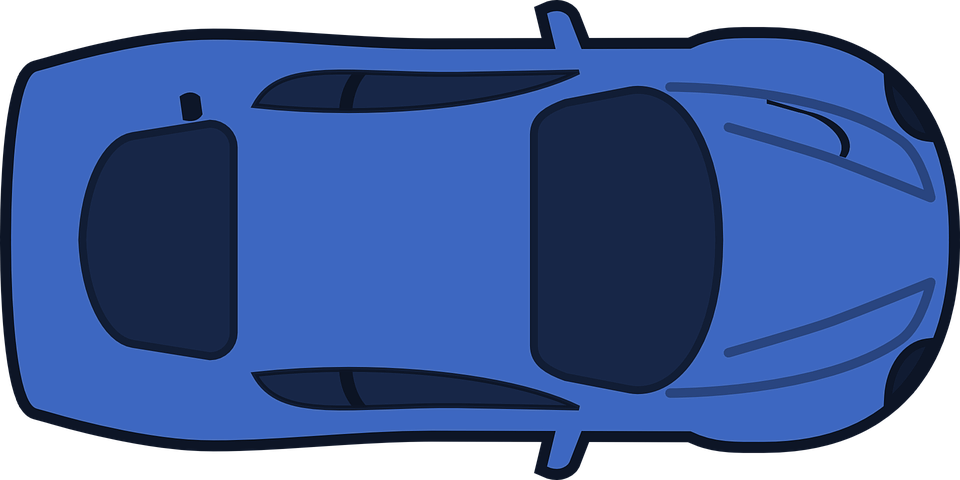
\includegraphics[width=.18\textwidth, angle=-90]{figures/target_car_top_down.png}};
% 	\node (tc_text2) [right=of target_car_2] {Car 2};
	
% 	\node[inner sep=0pt] (target_car_1) at (0,-1.5)
% 	{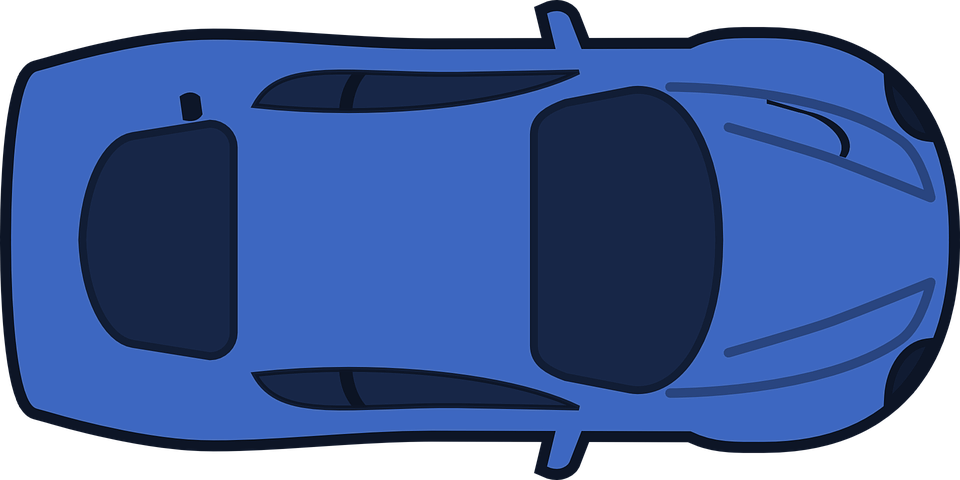
\includegraphics[width=.18\textwidth, angle=-90]{figures/target_car_top_down.png}};
% 	\node (tc_text1) [right=of target_car_1] {Car 1};

% \end{tikzpicture}
% \caption{Observations that makes the state}
% \label{fig:intersection_scenario}
% \end{figure}

\begin{figure}
\centering
\begin{tikzpicture}
	\def\xstart{-7};

	% Crossing
	\draw[line width=0.5mm] (\xstart, 1) -- (-1, 1) -- (-1, 5);
	\draw[line width=0.5mm] (\xstart, -1) -- (-1, -1) -- (-1, -2);
	\draw[line width=0.5mm] (1, 5) -- (1, 1) -- (3, 1);
	\draw[line width=0.5mm] (1, -2) -- (1, -1) -- (3, -1);
	
	% cars
	\node[inner sep=0pt] (ego_car) at (-6,0)
	{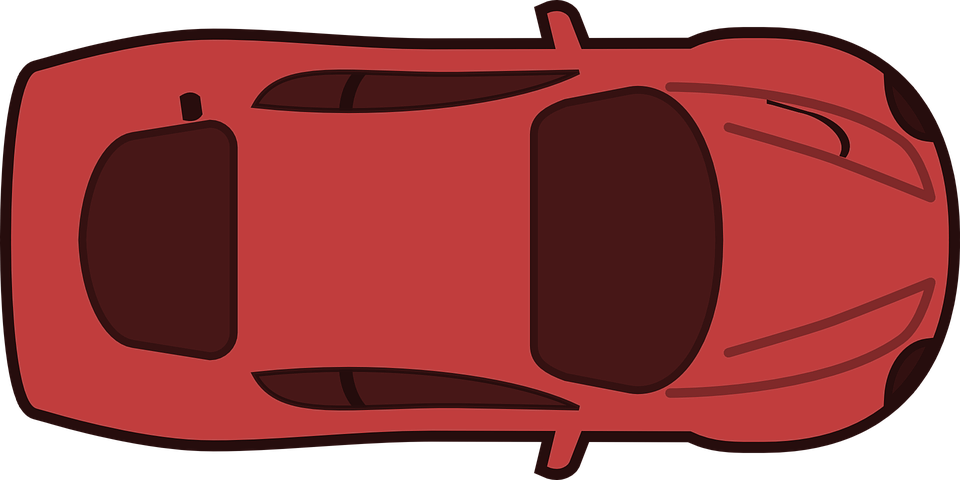
\includegraphics[width=.18\textwidth, angle=0]{figures/ego_car_top_down.png}};
	\node[inner sep=0pt] (target_car) at (0,4)
	{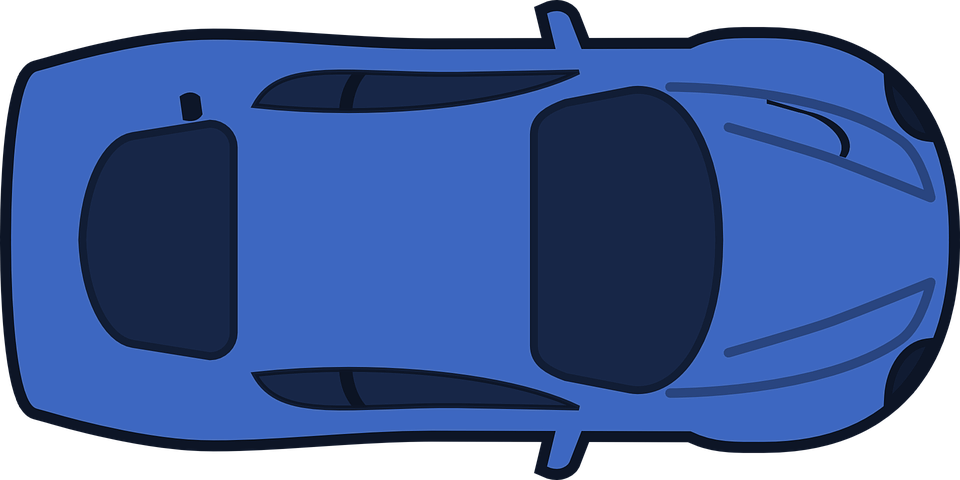
\includegraphics[width=.18\textwidth, angle=-90]{figures/target_car_top_down.png}};

\end{tikzpicture}
\caption{}
\label{fig:intersection_scenario}
\end{figure}


Figure \ref{fig:intersection_scenario} shows a simple intersection with one crossing point. 
\tommy{show examples of intersections.}
\tommy{zone 0 - after intersection, zone 1 - conflict zone, zone 2 - right before the intersection, zone 3 - first obsereved interstion to zone 2}



\section{State space}
From Section~\ref{sec:background_mdp}, the state space contains all the information necessary about the agent and environment to be able to transition to any given state. In the scenario from Figure~\ref{fig:intersection_scenario}, the red car on the horizontal lane represents the ego vehicle and the blue cars on the vertical lane are the other vehicels. 
Let's start by defining the information needed. Starting with the terminal states: goal, to know if ego vehicles has crossed the intersection and reached the goal. The distance from ego to goal $p_{goal}$ is needed. For collision, the position of all surrounding traffic participants and a description of the intersection itself is necessary. Instead of using a Cartesian coordinate system, I propose using relative distance measures instead. This way, states describing the intersection and its participants are generalizable to different intersection designs, e.g., the angle of incidence and number of crossing points. 
Then, the velocity and acceleration of all the traffic participants is necessary to be able to predict what position they will be in the next state. Finally, the intention of all the other participants. This state is necessary to efficently navigate through an interdection. \paperBelief shows a comparision between two fully observable \gls{mdp}s, one with intention and the other one without and the results show that having an intention state reduce number of collisions. 
\paperLSTM proposed the first set of states. %The states describing ego and other vehicle are spearated. Repeat the states for each other vehicle we observe. 
\tommy{Coordinate system, distances to intersection, position, velocity and accelration of other vehicles. abstract away the information about traffic lights, traffic signs, as intention}

\section{Action space}
\tommy{options, take way, give way, follow car}
One of the limitations of deep Q-learning is that the action space has to be discreet. In other work it is common to set the action space to diffecnt acceleration request. However, I propose using short term goals as actions, this is also refered to as options \cite{options}. The short term goals are high level objectives like stop at the start of the intersection, follow car with id 1 or drive through the intersection at the reference speed. 
This high level action is then sent to a sliding mode controller that generates an acceleration. 
In \paperMPC the actions is sent to a \gls{mpc} to generate a velocity profile that considers consecutive intersection points, this appoach is decribed in more detail in Chapter~\ref{ch:mpc}.  

\section{Transistion model}
In this work the transision model is not known to the agent and \gls{rl} is used to learn this model through experience, by taking actions at different states in an environment and recording the reward and what state the agent transition into.
the environment in this work is a simulator and the main thing the agent is traying to learn is the transision of the other vehicles which depends on their intentions. 
The intentions are models as predetermined actions while folloing a \gls{idm} ontop of that. This makes the interaction between cars more complicated. 
\tommy{IDM, and other agents behaviors/intentions.}
\paperLSTM random parameters, speeds and spawn rates. 
\paperMPC cautious, give way, take way


\subsection{Simulation scenarios or simulator}
parameters, randomized cars. Behaviors. spawn rates and more. up to four cars. 
singla crossing, double crossing, 

\section{Observation model}
The observation model can be interpeted as the noise from the sensors, \paperLSTM assumes perfect sensing while \paperBelief has some added noise to the observed states. 
The observation space is usually the same as the state space without the intention state. Because there are no sensors that can detect other drivers intentions. 
\tommy{Everything in the state space except intention. Everything that is observable through the sensors in the car. }

\section{Reward function}
Designing the reward model from the objective the agent are trying to achieve. this is not the optimal values. Starting of a relative reward difference around 0 and 1. Then hand tune to get a performance close to the desired outcome. 
All papers formulated the reward based on the terminal states: goal, collision and timeout. 
\paperLSTM and \paperMPC has a continious negative reward for change in acceleration to punish jerk that would come from changing between actions that would make it uncomfortable for the passengers. 
\paperLSTM also gives a relative large negative reward for choosing to follow a car that does not exist. 
\section{Discussion}
Why is it hard. 
\tommy{zone 0 - after intersection, zone 1 - conflict zone, zone 2 - right before the intersection, zone 3 - first obsereved interstion to zone 2}

\begin{figure}\label{fig:zones}
	\mbox{\parbox{\textwidth}{
		\centering
		\begin{tikzpicture}
			\def\xstart{-7};

			\coordinate (p) at (3,0);
			\foreach \n/\w/\c in {z0/2/green,z1/2/red,z2/2.5/orange,z3/3.5/blue}{
				\node[rectangle,
				draw=none,
				anchor=east,
				text = black,
				fill = \c!60,
				minimum width = \w cm, 
				minimum height = 2cm] 
				(n) at (p) {\Huge \n};
				
				\coordinate (p) at (n.west);
			}

			% Crossing
			\draw[line width=0.5mm] (\xstart, 1) -- (-1, 1) -- (-1, 5);
			\draw[line width=0.5mm] (\xstart, -1) -- (-1, -1) -- (-1, -2);
			\draw[line width=0.5mm] (1, 5) -- (1, 1) -- (3, 1);
			\draw[line width=0.5mm] (1, -2) -- (1, -1) -- (3, -1);
			
			% cars
			\node[inner sep=0pt] (ego_car) at (-7,0)
			{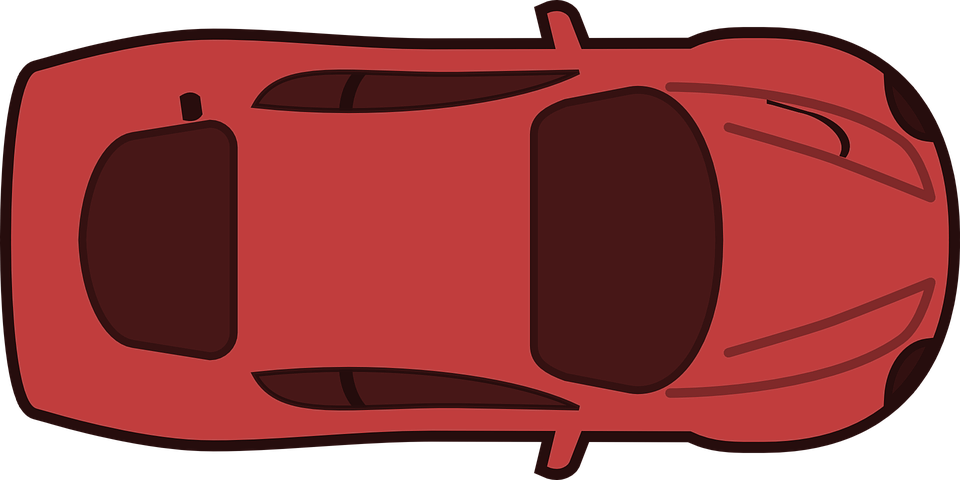
\includegraphics[width=.18\textwidth, angle=0]{figures/ego_car_top_down.png}};
			\node[inner sep=0pt] (target_car) at (0,4)
			{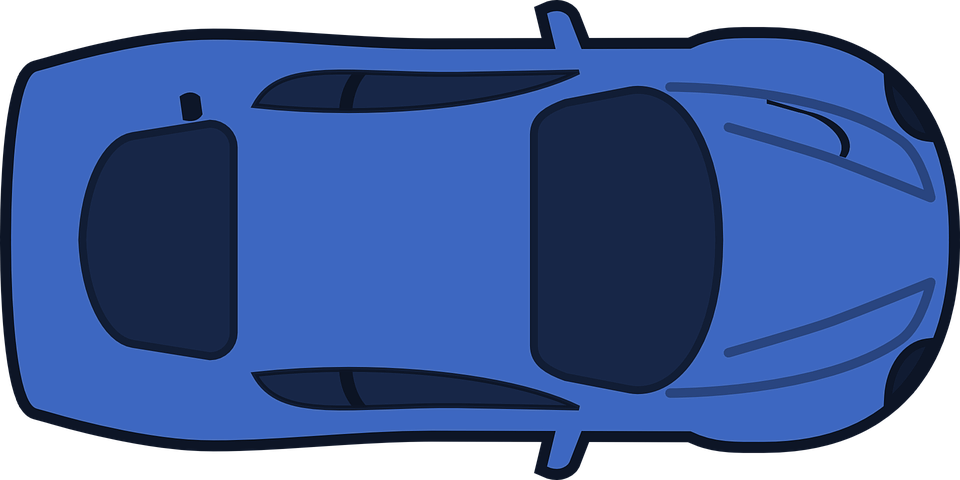
\includegraphics[width=.18\textwidth, angle=-90]{figures/target_car_top_down.png}};

	\end{tikzpicture}
	}}
	\caption{Intersection scenario divided into zones describing what is required of the decision maker in different zones}
	
\end{figure}

With the \gls{mdp}, defined a typical intersection can be described as in Figure \ref{fig:zones}. From the figure the path of the ego vehicle can be divided into four zones. Starting from the end, zone 0 is the "safe zone" where the ego is our of danger and can return to nominal driving. Zone 1 is the conflict zone, this is where there is a possibility to collide with another vehicle. Zone 2 is critical decision zone, where this is the last chance the vehicle has to stop or cross. The size of this zone is defined as the minimal distance the car needs to come to a complete stop to the start of the conflict zone. The final zone is zone 3, the information gathering zone, and is the furthest from the intersection and where the agent can observe the scenario and the other vehicles behavior over time. 

the goal is to reach zone 0, 
to do this the agent would want to minimize the time in zone 1, if there is chance of intersection with another car.
Because our actions are formulated as options and designed to be conformtable with lower acceleration rates. The size of zone 2 is dependent on the vehicels current speed, which is dependent on how the vehicle behaved in zone 3. 
Now there are two conflicting strategies, to minimize time in zone 1 the agent wants a high speed coming into the intersection. while it would want a low speed to shorten the zone 2 and the critical decision. 

If the intention of the other vehicles is known the stochasticity in zone 1 would be gone and the problem becomes a scheduling problem of creating a velocity profile that minimizes the time to cross.  

